%!TEX encoding = UTF-8 Unicode
%!TEX root = ../algos-geometriques.tex


\chapter{Rectangle}

Il s'agit de rectangles d'orientation quelconque, ce qui généralise les rectangles « horizontaux » du \refChapterPage{rectangleHorizontal}.

Un rectangle est caractérisé par :
\begin{itemize}
  \item son centre $C$ ;
  \item son angle $\alpha$ avec l'horizontal ;
  \item sa largeur $l$ ;
  \item sa hauteur $h$.
\end{itemize}

\begin{center}
  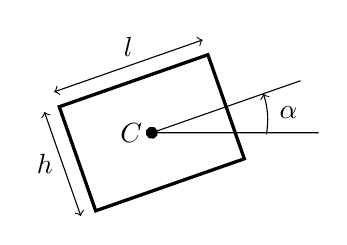
\begin{tikzpicture}[rotate=19.29]
    \draw[very thick] (0, -.2) rectangle (2, 1.2) ;
    \draw[thin] (1, .5) -- ++ (2, 0) ;
    \draw[thin] (1, .5) -- ++ (2, -0.7) ;
    \draw[fill] (1, 0.5) circle (2pt) ;
    \draw[left] (1, 0.5) node {$C$} ;
    \draw[<->] (-.2, -.2) -- ++ (0, 1.4) ;
    \draw[left] (-.2, .5) node {$h$} ;
    \draw[<->] (0, 1.4) -- ++ (2, 0) ;
    \draw[above] (1, 1.4) node {$l$} ;
    \draw[<-] (2.5, 0.5) arc (0:-30:1) ;
    \draw[right] (2.5, .25) node {$\alpha$} ;
  \end{tikzpicture}
\end{center}

C'est un type qui n'existe pas en Cocoa, il est défini dans \texttt{ElCanari} par une structure non mutable. Ce type est implémenté dans \texttt{CanariRect.swift}.

\begin{lstlisting}
struct CanariRect {
  let center : CGPoint
  let angle : CGFloat // In radians
  let size : CGSize
  
  ...
}
\end{lstlisting}





\section{Construction à partir d'un rectangle horizontal (\texttt{CGRect})}

\begin{lstlisting}
  init (cgrect : CGRect) {
    center = CGPoint (x: NSMidX (cgrect), y: NSMidY (cgrect))
    size = cgrect.size
    angle = 0.0
  }
\end{lstlisting}






\section{Construction à partir de deux points et d'une hauteur}

\begin{center}
  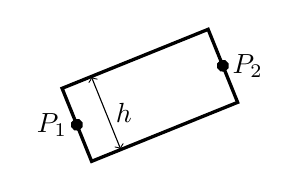
\begin{tikzpicture}[rotate=22.0]
    \draw[very thick] (0, 0) rectangle (2, 1) ;
    \draw[fill] (0, 0.5) circle (2pt) ;
    \draw[fill] (2, 0.5) circle (2pt) ;
    \draw[left] (0, 0.5) node {$P_1$} ;
    \draw[right] (2, 0.5) node {$P_2$} ;
    \draw[<->] (0.4, 0) -- ++ (0, 1) ;
    \draw[right] (0.4, .5) node {$h$} ;
  \end{tikzpicture}
\end{center}


\begin{lstlisting}
  init (from p1 : CGPoint, to p2 : CGPoint, height : CGFloat) {
    center = CGPoint (x: (p1.x + p2.x) * 0.5, y: (p1.y + p2.y) * 0.5)
    size = CGSize (width: CGPoint.distance (p1, p2), height: height)
    angle = CGPoint.angleInRadian (p1, p2)
  }
\end{lstlisting}






\section{Construction à partir du centre, angle et taille}

\begin{lstlisting}
  init (center : CGPoint, size : CGSize, angle : CGFloat) {
    self.center = center
    self.size = size
    self.angle = angle
  }
\end{lstlisting}






\section{Cercle inscrit}

\begin{center}
  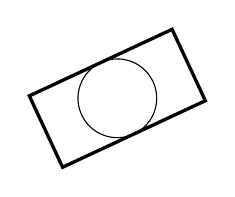
\begin{tikzpicture}[rotate=25]
    \draw[very thick] (0, 0) rectangle (2, 1) ;
    \draw[thin] (1, 0.5) circle (0.5cm) ;
  \end{tikzpicture}
\end{center}

\begin{lstlisting}
  func inscribedCircle () -> CanariCircle {
    let radius = min (size.width, size.height) / 2.0
    return CanariCircle (center: self.center, radius: radius)
  }
\end{lstlisting}






\section{Cercle circonscrit}

\begin{center}
  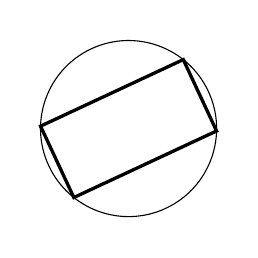
\begin{tikzpicture}[rotate=25]
    \draw[very thick] (0, 0) rectangle (2, 1) ;
    \draw[thin] (1, 0.5) circle (1.118cm) ;
  \end{tikzpicture}
\end{center}

\begin{lstlisting}
  func circumCircle () -> CanariCircle {
    let radius = sqrt (size.width * size.width + size.height * size.height) / 2.0
    return CanariCircle (center: self.center, radius: radius)
  }
\end{lstlisting}







\section{Inclusion d'un point}

Le test d'inclusion d'un point est plus délicat à mettre au point, bien que le code résultant soit court. Le principe est d'effectuer un changement de repère, de façon à obtenir les coordonnées du point testé dans le repère lié au rectangle, qui devient alors un rectangle horizontal. Tester l'appartenance du point devient élémentaire dans ce nouveau repère. 

\begin{center}
  \def\angle{19.29}
  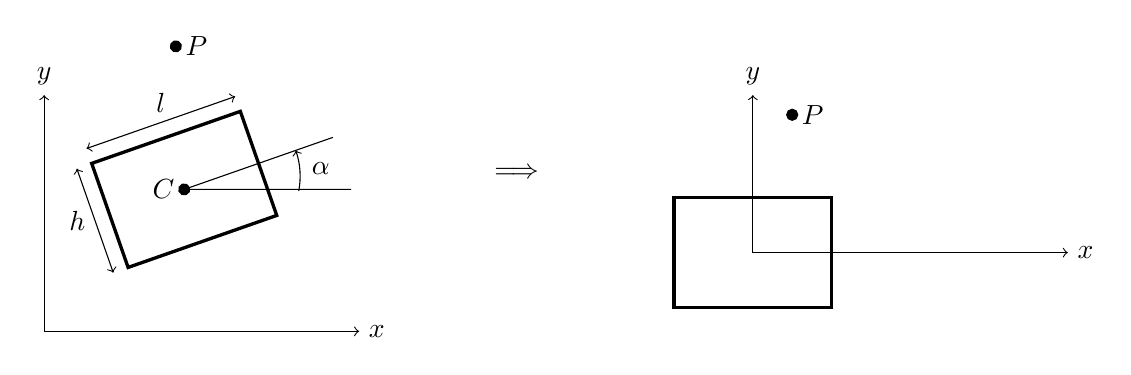
\begin{tikzpicture}
    \begin{scope}[rotate=\angle]
      \begin{scope}[rotate=-\angle]
        \draw[thin,->] (-1, -1) -- ++ (4, 0) node[right] {$x$} ;
        \draw[thin,->] (-1, -1) -- ++ (0, 3) node[above] {$y$} ;
      \end{scope}
      \draw[fill] (1.5, 2.25) circle (2pt) node[right] {$P$} ;
      \draw[very thick] (0, -.2) rectangle ++ (2, 1.4) ;
      \draw[thin] (1, .5) -- ++ (2, 0) ;
      \draw[thin] (1, .5) -- ++ (2, -0.7) ;
      \draw[fill] (1, 0.5) circle (2pt) ;
      \draw[left] (1, 0.5) node {$C$} ;
      \draw[<->] (-.2, -.2) -- ++ (0, 1.4) ;
      \draw[left] (-.2, .5) node {$h$} ;
      \draw[<->] (0, 1.4) -- ++ (2, 0) ;
      \draw[above] (1, 1.4) node {$l$} ;
      \draw[<-] (2.5, 0.5) arc (0:-30:1) ;
      \draw[right] (2.5, .25) node {$\alpha$} ;
    \end{scope}
    \draw (5, 1) node {$\Longrightarrow$} ;
    \begin{scope}[xshift=8cm]
      \draw[thin,->] (0, 0) -- ++ (4, 0) node[right] {$x$} ;
      \draw[thin,->] (0, 0) -- ++ (0, 2) node[above] {$y$} ;
      \draw[very thick] (-1, -.7) rectangle ++ (2, 1.4) ;
      \draw[fill] (0.5, 1.75) circle (2pt) node[right] {$P$} ;
    \end{scope}
  \end{tikzpicture}
\end{center}


\begin{lstlisting}
  func contains (point p : CGPoint) -> Bool {
    let tr = CGAffineTransform (rotationAngle: -angle)
            .translatedBy (x:-center.x, y:-center.y)
    let point = p.applying (tr)
    return (abs (point.x) <= (size.width * 0.5))
        && (abs (point.y) <= (size.height * 0.5))
  }
\end{lstlisting}







\section{Coordonnées des sommets}

La fonction suivante retourne dans un tableau les quatre sommets du rectangle. Le tableau est ordonné, on parcourt les sommets dans le sens trigonométrique.

\begin{lstlisting}
  func vertices () -> [CGPoint] { // Returns the four vertices in counterclock order
    let cosSlash2 = cos (angle) / 2.0
    let sinSlash2 = sin (angle) / 2.0
    let widthCos  = size.width  * cosSlash2
    let widthSin  = size.width  * sinSlash2
    let heightCos = size.height * cosSlash2
    let heightSin = size.height * sinSlash2
    return [
      CGPoint (x: center.x + widthCos - heightSin, y: center.y + widthSin + heightCos),
      CGPoint (x: center.x - widthCos - heightSin, y: center.y - widthSin + heightCos),
      CGPoint (x: center.x - widthCos + heightSin, y: center.y - widthSin - heightCos),
      CGPoint (x: center.x + widthCos + heightSin, y: center.y + widthSin - heightCos)
    ]
  }
\end{lstlisting}







\section{Intersection avec un cercle}

Il y a intersection si :
\begin{itemize}
  \item si le cercle contient le centre du rectangle ;
  \item ou si le rectangle contient le centre du cercle ;
  \item ou, à défaut, si le cercle présente une intersection avec l'un des quatre côtés du rectangle.
\end{itemize}


\begin{lstlisting}
  func intersects (circle : CanariCircle) -> Bool {
  //--- Intersection if circle contains rectangle center
    var intersects = CGPoint.distance (self.center, circle.center) <= circle.radius
  //--- Intersection if rectangle contains circle center
    if !intersects {
      intersects = self.contains (point: circle.center)
    }
  //--- Test intersection between circle and rectangle edge
    if !intersects {
      let vertices = self.vertices ()
      var i = 0
      while !intersects && (i < vertices.count) {
        intersects = circle.intersects (segmentFrom: vertices [i],
                                        to: vertices [(i+1) % vertices.count])
        i += 1
      }
    }
    return intersects
  }
\end{lstlisting}






\section{Intersection avec un autre rectangle}

La méthode qui fait autorité est la méthode dite de \emph{séparation d'axes}. Elle est illustrée dans la video \url{https://www.youtube.com/watch?v=WBy6AveIRRs}. En résumé, il n'y a pas intersection si il existe une droite pour laquelle un rectangle est complètement contenu dans un demi-plan, et l'autre rectangle complètement contenu dans l'autre demi-plan.

\begin{center}
  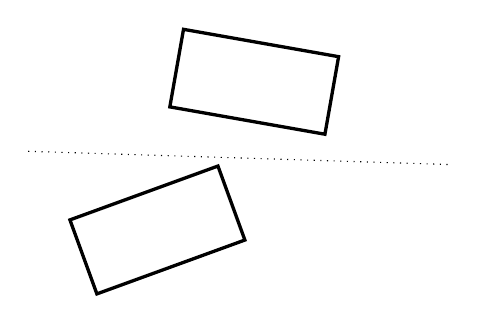
\begin{tikzpicture}[rotate=20]
    \draw[very thick] (0, 0) rectangle (2, 1) ;
    \begin{scope}[rotate=-30]
      \draw[very thick] (0.5, 2.5) rectangle ++ (2, 1) ;
    \end{scope}
    \draw[thin,dotted] (-.2, 2) -- ++ (5, -2) ;
  \end{tikzpicture}
\end{center}

L'intérêt de la méthode est que l'on n'a pas besoin de construire une telle droite, qui d'ailleurs n'est pas unique dans le cas général.

Il faut commencer par construire les sommets des rectangles.

\begin{center}
  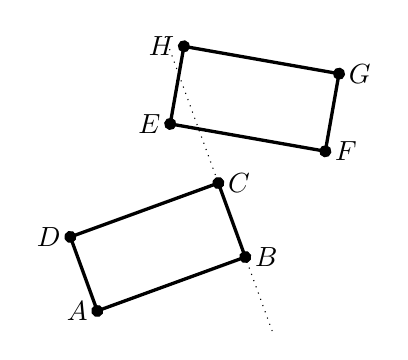
\begin{tikzpicture}[rotate=20]
    \draw[thin,dotted] (2, -1) -- ++ (0, 4) ;
    \draw[very thick] (0, 0) rectangle (2, 1) ;
    \draw[fill] (0, 0) circle (2pt) node[left] {$A$} ;
    \draw[fill] (2, 0) circle (2pt) node[right] {$B$} ;
    \draw[fill] (2, 1) circle (2pt) node[right] {$C$} ;
    \draw[fill] (0, 1) circle (2pt) node[left] {$D$} ;
    \begin{scope}[rotate=-30]
      \draw[very thick] (0.5, 2.5) rectangle ++ (2, 1) ;
      \draw[fill] (0.5, 2.5) circle (2pt) node[left] {$E$} ;
      \draw[fill] (2.5, 2.5) circle (2pt) node[right] {$F$} ;
      \draw[fill] (2.5, 3.5) circle (2pt) node[right] {$G$} ;
      \draw[fill] (0.5, 3.5) circle (2pt) node[left] {$H$} ;
    \end{scope}
  \end{tikzpicture}
\end{center}

Ensuite, pour chaque côté du premier rectangle, on effectue le \emph{test de séparation} : il est positif si les quatre sommets de l'autre rectangle sont « de l'autre côté ». Par exemple, on considère le coté $BC$, qui définit une droite qui partage le plan en deux. Par la fonction \texttt{CGPoint.product}, on calcule la composante verticale de $\overrightarrow{BC} \wedge \overrightarrow{CD}$ : son signe caractérise le demi-plan du premier rectangle. On calcule ensuite la composante verticale de $\overrightarrow{BC} \wedge \overrightarrow{CP}$, pour les quatre sommets $P$ du second rectangle. On obtient un signe contraire pour les sommets $F$, $G$, $H$, mais le même signe pour le sommet $E$, ce qui fait échouer le test de séparation.

Le test de séparation réussit en considérant le segment $EF$ :

\begin{center}
  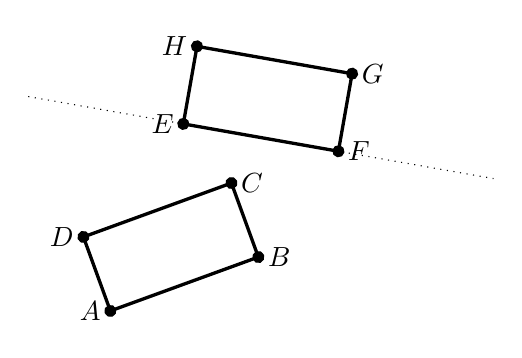
\begin{tikzpicture}[rotate=20]
    \draw[very thick] (0, 0) rectangle (2, 1) ;
    \draw[fill] (0, 0) circle (2pt) node[left] {$A$} ;
    \draw[fill] (2, 0) circle (2pt) node[right] {$B$} ;
    \draw[fill] (2, 1) circle (2pt) node[right] {$C$} ;
    \draw[fill] (0, 1) circle (2pt) node[left] {$D$} ;
    \begin{scope}[rotate=-30]
      \draw[thin,dotted] (-1.5, 2.5) -- ++ (6, 0) ;
      \draw[very thick] (0.5, 2.5) rectangle ++ (2, 1) ;
      \draw[fill] (0.5, 2.5) circle (2pt) node[left] {$E$} ;
      \draw[fill] (2.5, 2.5) circle (2pt) node[right] {$F$} ;
      \draw[fill] (2.5, 3.5) circle (2pt) node[right] {$G$} ;
      \draw[fill] (0.5, 3.5) circle (2pt) node[left] {$H$} ;
    \end{scope}
  \end{tikzpicture}
\end{center}

Il faut donc effectuer le test de séparation pour chaque côté du premier rectangle {\bf et} chaque côté du second rectangle. Il y a intersection si {\bf tous} les tests de séparation échouent, donc pas d'intersection si un des tests réussit.

Il est indispensable de faire les tests pour les deux rectangles : en effet, ils peuvent échouer pour chaque côté du premier rectangle, alors qu'il n'y a pas intersection. Par exemple dans la figure suivante, les quatre tests d'isolation échouent pour les quatre côtés du rectangle $ABCD$.

\begin{center}
  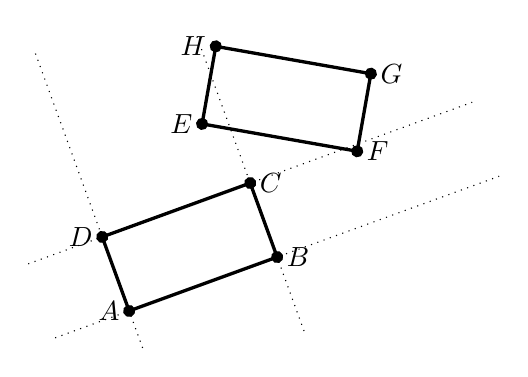
\begin{tikzpicture}[rotate=20]
    \draw[thin,dotted] (2, -1) -- ++ (0, 4) ;
    \draw[thin,dotted] (0, -.5) -- ++ (0, 4) ;
    \draw[thin,dotted] (-1, 0) -- ++ (6, 0) ;
    \draw[thin,dotted] (-1, 1) -- ++ (6, 0) ;
    \draw[very thick] (0, 0) rectangle (2, 1) ;
    \draw[fill] (0, 0) circle (2pt) node[left] {$A$} ;
    \draw[fill] (2, 0) circle (2pt) node[right] {$B$} ;
    \draw[fill] (2, 1) circle (2pt) node[right] {$C$} ;
    \draw[fill] (0, 1) circle (2pt) node[left] {$D$} ;
    \begin{scope}[rotate=-30]
      \draw[very thick] (0.5, 2.5) rectangle ++ (2, 1) ;
      \draw[fill] (0.5, 2.5) circle (2pt) node[left] {$E$} ;
      \draw[fill] (2.5, 2.5) circle (2pt) node[right] {$F$} ;
      \draw[fill] (2.5, 3.5) circle (2pt) node[right] {$G$} ;
      \draw[fill] (0.5, 3.5) circle (2pt) node[left] {$H$} ;
    \end{scope}
  \end{tikzpicture}
\end{center}


Voici le code de la fonction.

\begin{lstlisting}
  func intersects (rect : CanariRect) -> Bool {
  //--- Method of separating axes (https://www.youtube.com/watch?v=WBy6AveIRRs)
    var intersects = true
    let vertices1 = self.vertices ()
    let vertices2 = rect.vertices ()
    do{
      var i = 0
      while intersects && (i < vertices1.count) {
        let ref = CGPoint.product (vertices1 [i],
                                   vertices1 [(i+1) % vertices1.count],
                                   vertices1 [(i+2) % vertices1.count])
        var outside = true
        var j = 0
        while outside && (j < vertices2.count) {
          let test = CGPoint.product (vertices1 [i],
                                      vertices1 [(i+1) % vertices1.count],
                                      vertices2 [j])
          outside = (ref * test) < 0.0
          j += 1
        }
        intersects = !outside
        i += 1
      }
    }
  //---
    if intersects {
      var i = 0
      while intersects && (i < vertices2.count) {
        let ref = CGPoint.product (vertices2 [i],
                                   vertices2 [(i+1) % vertices2.count],
                                   vertices2 [(i+2) % vertices2.count])
        var outside = true
        var j = 0
        while outside && (j < vertices1.count) {
          let test = CGPoint.product (vertices2 [i],
                                      vertices2 [(i+1) % vertices2.count],
                                      vertices1 [j])
          outside = (ref * test) < 0.0
          j += 1
        }
        intersects = !outside
        i += 1
      }
    }
  //---
    return intersects
  }
\end{lstlisting}

